
\chapter{Filling of gaps in meteorological time series (\software{meteofill})} \label{chap:meteofill}
\renewcommand{\tabdir}{chapters/meteofill/tab}
\renewcommand{\figdir}{chapters/meteofill/fig}

%%%%%%%%%%%%%%%%%%%%%%%%%%%%%%%%%%%%%%%%%%%%%%%%%%%%%%%%%%%%%%%%%%%%%%%%%%%%%%%%
%%%%%%%%%%%%%%%%%%%%%%%%%%%%%%%%%%%%%%%%%%%%%%%%%%%%%%%%%%%%%%%%%%%%%%%%%%%%%%%%
%%%%%%%%%%%%%%%%%%%%%%%%%%%%%%%%%%%%%%%%%%%%%%%%%%%%%%%%%%%%%%%%%%%%%%%%%%%%%%%%
\section{Purpose} \label{sec:meteofill:purpose}
For hydrological modeling, time series of meteorological variables are required. Besides rainfall, this usually includes variables like temperature, radiation, humidity, windspeed, and possibly air pressure. The time series of meteorological observations often containg some (or many) missing values due to failure of sensors, power blackout, errors in transmission and recording of data and various other causes.

Internally, all hydrological models require continuous (\ie{} gap-free) time series of the meteorological forcing variables. This requirement can be fulfilled in two different ways. In the first strategy (\figref{fig:meteofill:fill_alternatives}, left) the model reads the incomplete series and must fill the gaps internally. The second strategy (\figref{fig:meteofill:fill_alternatives}, right) uses an external pre-processor to complete the information before calling the model.

The second approach has a number of advantages listed below:

\begin{itemize}
  \item Models are often run many times using the same input data set (for example in calibration or uncertainty analysis). It would be a massive waste of computer time to repeatedly pre-process the time series input in every single run.
  \item Separating the time series pre-processor from the actual model makes the software more modular which is advantageous in terms of re-use and maintenance.
\end{itemize}

\begin{figure}
  \centering
  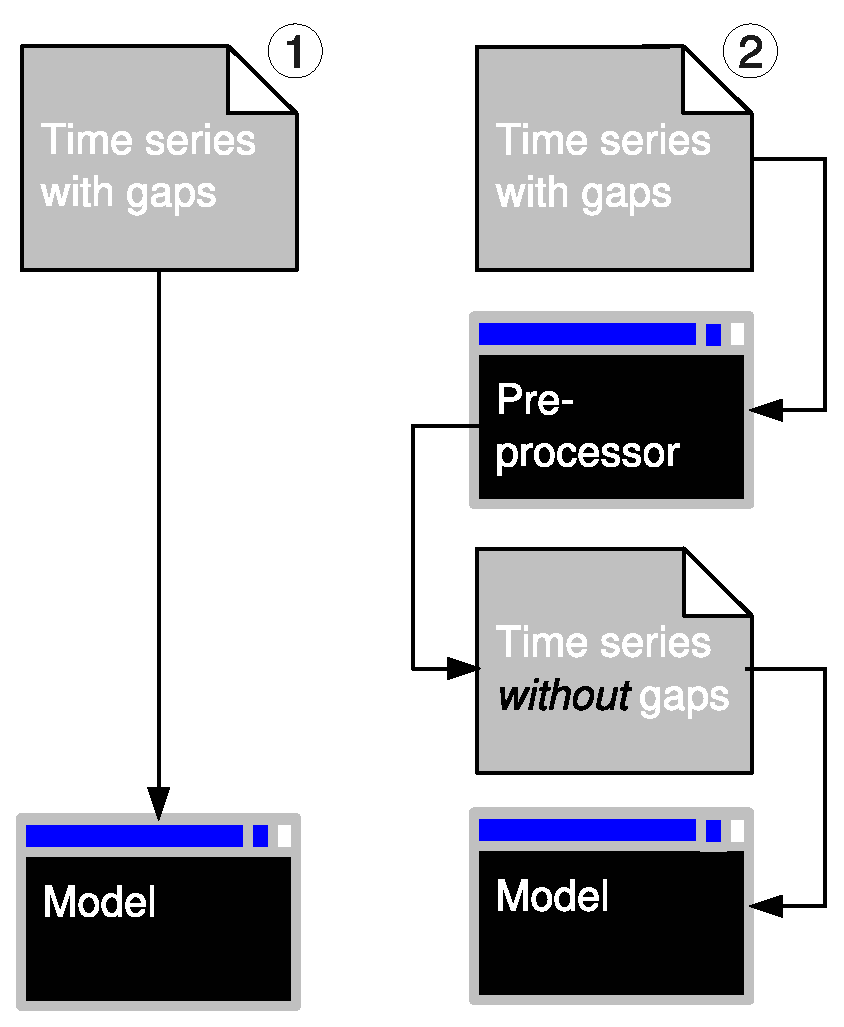
\includegraphics[width=0.65\columnwidth]{\figdir/fill_alternatives.eps}
  \caption{Alternative strategies to handle gaps a model's input time series. \label{fig:meteofill:fill_alternatives}}
\end{figure}

\software{meteofill} is designed for the second approach (\figref{fig:meteofill:fill_alternatives}, right). It is a pre-processor to produce gap-free time series from observation data.

The methodology used by \software{meteofill} is built on a space-for-time trade approach (see \secref{sec:meteofill:method}). It requires that observation data are available for \emph{multiple stations}. Using \software{meteofill} to fill gaps in a time series of observations at a single location is technically possible but it is likely to give poor result (see details in \secref{sec:meteofill:filling}).

Note that, for \emph{spatially distributed} models, there are now \emph{two separate steps of spatial interpolation}. In the first step, \software{meteofill} is uses spatial interpolation to remove any gaps in the model's multi-location input time series. In the second step, typically called regionalization, the pre-processed multi-location data are then interpolated to the spatially distributed model objects.

This second interpolation step is typically fully independent of \software{meteofill} and may be carried out, for example, by the simulation model, or any geostatistical software.

It is also possible, however, to use \software{meteofill} to combine the two steps of spatial interpolation mentioned above. This is illustrated in \figref{fig:meteofill:possibleUses}.

In the left branch of \figref{fig:meteofill:possibleUses}, \software{meteofill} is used to fill the gaps in time series of actual observations made at real-world stations. The distributed model reads the pre-processed time series and performs the regionalization to the model objects internally. In this approach, the model reads a rather small amount of data from files which is efficient with respect to computation time and disk space. User's of \software{echse}-based models propably always want to use this approach.

The alternative is shown in the right branch of \figref{fig:meteofill:possibleUses}, where \software{meteofill} is used as an all-in-one interpolation tool. This is practically achieved by considering the locations of the model objects as 'normal' observation sites \emph{that never recorded any data}. This kind of usage may be problematic for models with many spatially distributed objects, in particular if longer time series are processed. The produced files may become extremely large, which may result in a massive slow-down of model performance and disk operations in general. Thus, the use of \software{meteofill} as an all-in-one interpolation tool is recommended in special cases only (small models, few time steps; see example in \figref{fig:meteofill:resid}).

\begin{figure*}
  \centering
  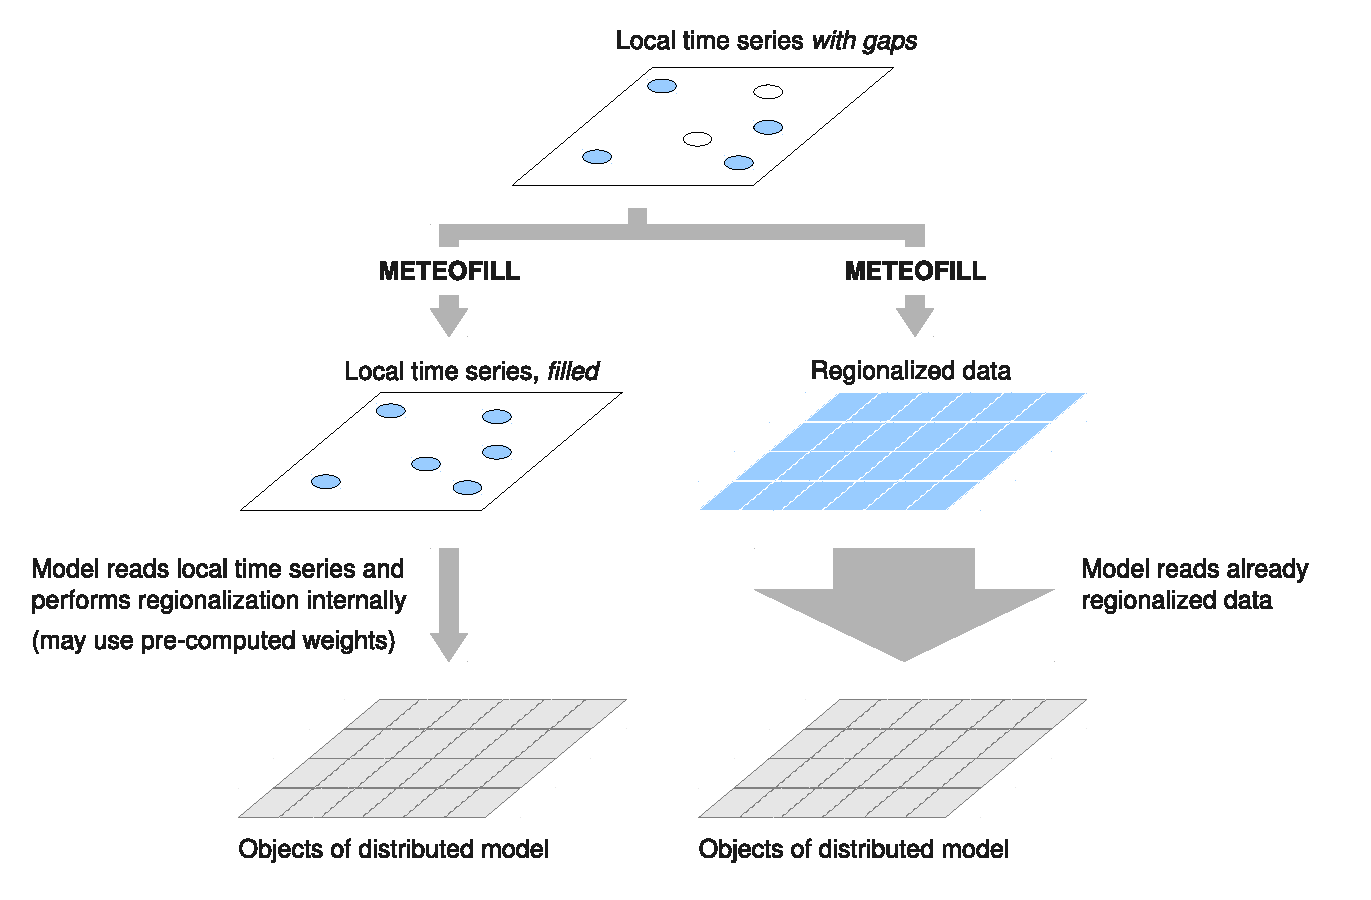
\includegraphics[width=0.8\textwidth]{\figdir/possibleUses.eps}
  \caption[Possible strategies of preparing the time series input of a spatially distributed model using \software{meteofill}]{Possible strategies of preparing the time series input of a spatially distributed model using \software{meteofill}. Whenever possible, the left branch should be preffered for performance reasons. \label{fig:meteofill:possibleUses}}
\end{figure*}

%%%%%%%%%%%%%%%%%%%%%%%%%%%%%%%%%%%%%%%%%%%%%%%%%%%%%%%%%%%%%%%%%%%%%%%%%%%%%%%%
%%%%%%%%%%%%%%%%%%%%%%%%%%%%%%%%%%%%%%%%%%%%%%%%%%%%%%%%%%%%%%%%%%%%%%%%%%%%%%%%
%%%%%%%%%%%%%%%%%%%%%%%%%%%%%%%%%%%%%%%%%%%%%%%%%%%%%%%%%%%%%%%%%%%%%%%%%%%%%%%%
\section{Methods} \label{sec:meteofill:method}

\subsection{Filling of gaps} \label{sec:meteofill:filling}
The approach taken by \software{meteofill} is best explained with an example (\figref{fig:meteofill:basics}). In order to substitute a missing data value (cross) by a reasonable estimate, one could, in theory:
\begin{enumerate}
  \item interpolate in time. For example, the missing value at location 3 in time step 4 could be substituted by interpolating between the values at the same location in time steps 3 and 5.
  \item assume persistence. For example, the missing value at location 3 in time step 4 could simply be substituted by the value from the previous time step (step 3, same location). This is actually a special case of interpolation in time, where the previous and next value are weighted with factors of 1 and 0, respectively.
  \item interpolate in space. For example, the missing values at locations 2 and 4 in time step 2 could be estimated by spatially interpolating the values from the remaining locations 1, 2, and 5 observed at the same time step.
  \item combine the ideas of spatial and temporal interpolation.
\end{enumerate}

\begin{figure}
  \centering
  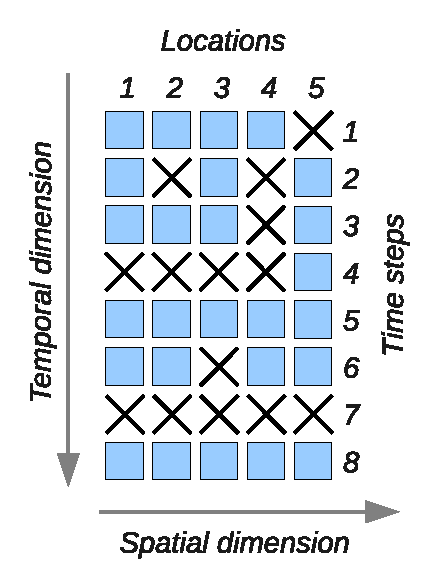
\includegraphics[width=0.55\columnwidth]{\figdir/basics.eps}
  \caption{Example of a multi-location times series of a meteorological variable with valid (squares) and missing data values (crosses). \label{fig:meteofill:basics}}
\end{figure}

The current version of \software{meteofill} primarily relies on \emph{spatial} interpolation, rather than interpolation in time. This can be summarizes by the following simple rules:
\begin{itemize}
  \item If, in a time step, a value is available at $n \geq 1$ location(s), missing data at the other $m$ locations are estimated by spatial interpolation (see \secsref{sec:meteofill:idw} and \ref{sec:meteofill:resid} for details). In the simplest case with $n=1$, the single observation is assumed to be valid globally.
  \item If, in a time step, no data are available at any location, persistence is assumed. Thus, for each location, the value (or estimate\footnote{If data are missing for a number of subsequent time steps}) from the previous time step is used (see \secref{sec:meteofill:hints:persistenceOptions} for practical advices).
\end{itemize}

After filling the gaps at all station in a time step $j$, the computation proceeds with time step $j+1$. This algorithm obviously requires that, in the very first time step, there is at least one location with a non-missing value.

\subsection{Inverse-distance approach} \label{sec:meteofill:idw}
The inverse-distance method (\eqnref{eqn:meteofill:idw}) is used to perform the spatial interpolation. It is a robust and computationally cheap method. To a limited extent, the spatial autocorrelation of the interpolated variable can be taken into account by adjustment of the exponent $p$ in \eqnref{eqn:meteofill:idw}.

\begin{equation}
y_k = \frac{\sum_{i=1}^{n} \left( y_i \cdot d(i,k)^{-p}\right)}{\sum_{i=1}^{n} \left( d(i,k)^{-p} \right)} \label{eqn:meteofill:idw}
\end{equation}

with

\begin{tabular}{lp{0.7\columnwidth}}
  $y_k$ & Value at the target location (index $k$). \\
  $y_i$ & Value at source location with index $i$. \\
  $d(i,k)$ & Distance between locations with indices $i$ and $k$. \\
  $p$ & Parameter (typically set to 2). \\
\end{tabular}

\medskip
For a particular target location (index $k$ in \eqnref{eqn:meteofill:idw}), the set of appropriate source locations (indices $1$ through $n$ in \eqnref{eqn:meteofill:idw}) is found by a sector search. Thus, the surrounding area of the location $k$ is dub-divided into a number of sectors and only the nearest source location is picked from each sector. This is illustrated in \figref{fig:meteofill:nearest}.

\begin{figure}
  \centering
  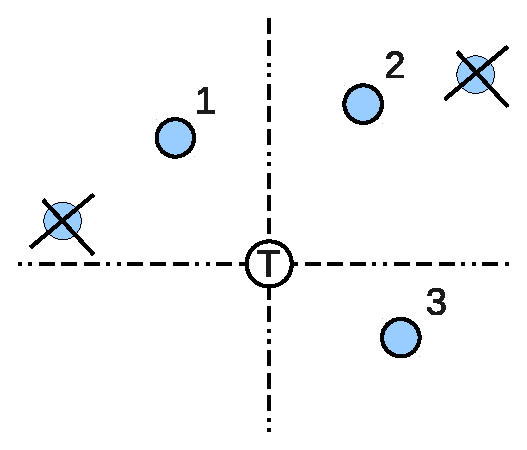
\includegraphics[width=0.55\columnwidth]{\figdir/interpolation_nearest.eps}
  \caption[Example of a sector search in spatial interpolation.]{Example of a sector search in spatial interpolation. From each of the four sectors, only the nearest station (1,2,3) is used in estimating the variable at the target location ($T$). Values at the crossed locations are neglected. \label{fig:meteofill:nearest}}
\end{figure}

Given a fixed number of sectors, the selection of the source location obviously depends on the orientation of the sectors. To achieve an optimum result, \software{meteofill} allows for testing different orientations by rotating the sectors (\figref{fig:meteofill:rotation}). From the tested orientations, \software{meteofill} uses the one where the cumulated distance between the target and the source locations is minimal.

\begin{figure}
  \centering
  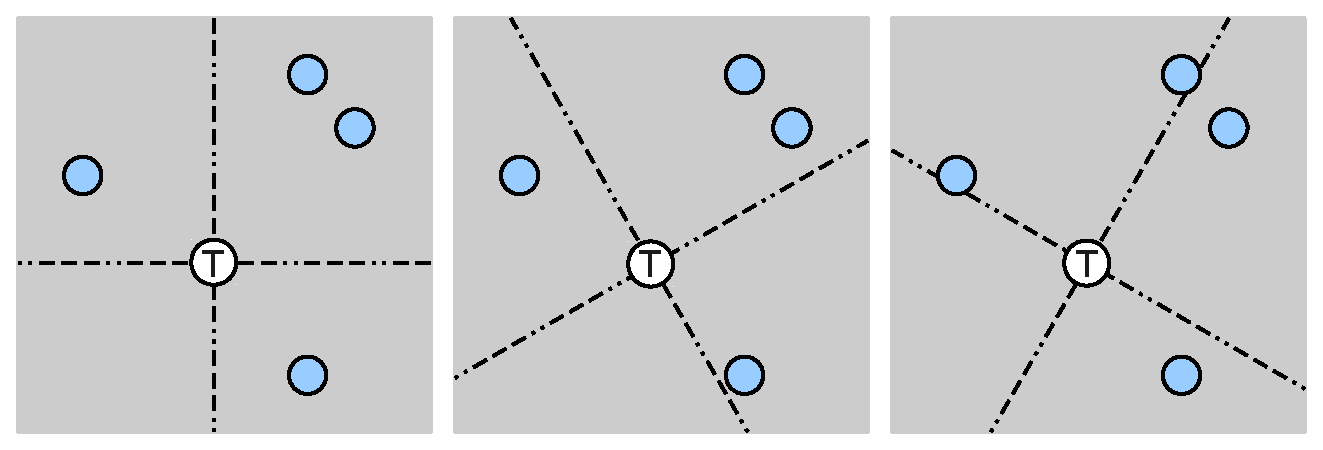
\includegraphics[width=0.95\columnwidth]{\figdir/interpolation_sectorrotation.eps}
  \caption[Example of sector rotation.]{Example of sector rotation. This example used a number of four sectors with 3 different orientations.  \label{fig:meteofill:rotation}}
\end{figure}

The selection of the appropriate source locations is the computationally most demanding step. This is especially so if both the number of target and source locations is large. Therefore, \software{meteofill} carries out a search for the source locations only
\begin{itemize}
  \item at the very beginning of the computation (first time step).
  \item if the set of locations with missing data has changed from the previous to the current time step.
\end{itemize}

\subsection{Residual interpolation} \label{sec:meteofill:resid}

The result of spatial interpolation can often be improved by using additional predictor variable(s). Values of these valiable(s) must be known at all source and target locations. For example, elevation my be a useful additional predictor when interpolating air pressure or temperature data. Two prominent approaches to spatial interpolation with additional predictors are (1) external drift Kriging and (2) residual interpolation.

\software{meteofill} supports the latter approach with the following settings/restrictions:
\begin{itemize}
  \item Only a \emph{single} predictor variable is supported.
  \item A \emph{linear} relation between the predictor and the interpolated variable is assumed.
  \item The \emph{additive} approach is used (not the alternative, multiplicative approach).
\end{itemize}

The basic algorithm of additive, uni-variate inverse-distance residual interpolation is summarized in \eqnsref{eqn:meteofill:resid_1} to \ref{eqn:meteofill:resid_3}

\begin{align}
y_k =& E_k + \frac{\sum_{i=1}^{n} \left( R_i \cdot d(i,k)^{-p}\right)}{\sum_{i=1}^{n} \left( d(i,k)^{-p} \right)} \label{eqn:meteofill:resid_1} \\
E_j =& a \cdot z_j + b \label{eqn:meteofill:resid_2} \\
R_i =& y_i - E_i \label{eqn:meteofill:resid_3}
\end{align}

with the additional symbols (cf. \eqnref{eqn:meteofill:idw})

\begin{tabular}{lp{0.7\columnwidth}}
  $E_j$ & Estimate of variable $y$ at an arbitrary location $j$ obtained from a linear model with the external predictor variable $z$ and empirical coefficients $a$ and $b$.  \\
  $R_i$ & Residual at a source location with index $i$. \\
\end{tabular}

The coefficients of the linear model (\eqnref{eqn:meteofill:resid_2}) are updated in every single time step. This is done using the data from all source locations (\ie{} all locations with valid data).

The linear correlation between the interpolated variable $y$ and the additional predictor variable $z$ may be more or less strong. In particular, the sign and quality of the correlation may be variable in time. Therefore, \software{meteofill} accepts a user-specified quality threshold, representing a minimum $R^2$. If the value of $R^2$ for the linear model (\eqnref{eqn:meteofill:resid_2}) is equal or greater than the user-specified threshold, residual interpolation is used (\eqnsref{eqn:meteofill:resid_1} to \ref{eqn:meteofill:resid_3}). Otherwise, in the case of a weak correlation, the plain inverse-distance method is applied (\eqnref{eqn:meteofill:idw}). The same is true if the number of data pairs for estimation of the linear model is lower than a user specified minimum sample size.

Residual interpolation is \emph{never} used if the threshold for $R^2$ is set to a value > 1 or if the minimum sample size is set to a value greater than the total number of locations.

In some cases, use of the linear model may result in undesired extrapolation effects. This is especially so, if
\begin{itemize}
  \item the range of possible values of the interpolated variable is limited. Example: Precipitation intensity cannot be negative.
  \item the value of the predictor variable $z$ at a target location is outside the range of $z$ values at the source locations. Example: Data are missing for a location at sea level and all available data correspond to elevations of 500--5000 meters.
\end{itemize}

In order to suppress such undesired results, \software{meteofill} allows for data truncation. The result values of residual interpolation are truncated if they are outside a user-specified range.

An example, illustrating the effect of residual interpolation in comparison with plain inverse-distance interpolation is shown in \figref{fig:meteofill:resid}.

\begin{figure*}
  \centering
  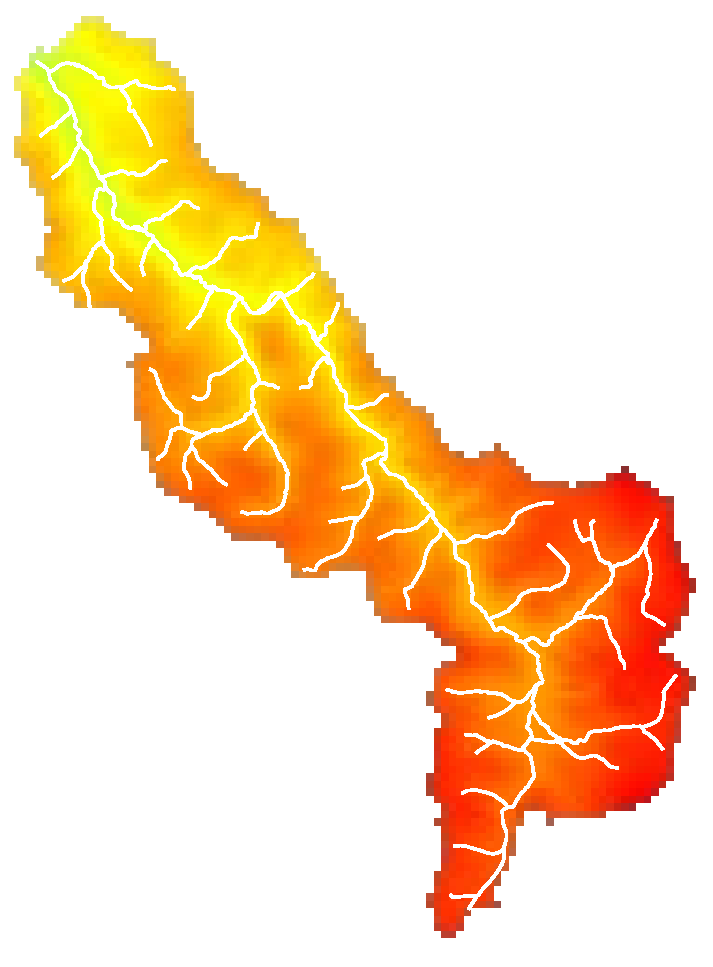
\includegraphics[width=0.3\textwidth, viewport=0 0 326 448, clip]{\figdir/demo/dem.eps}
  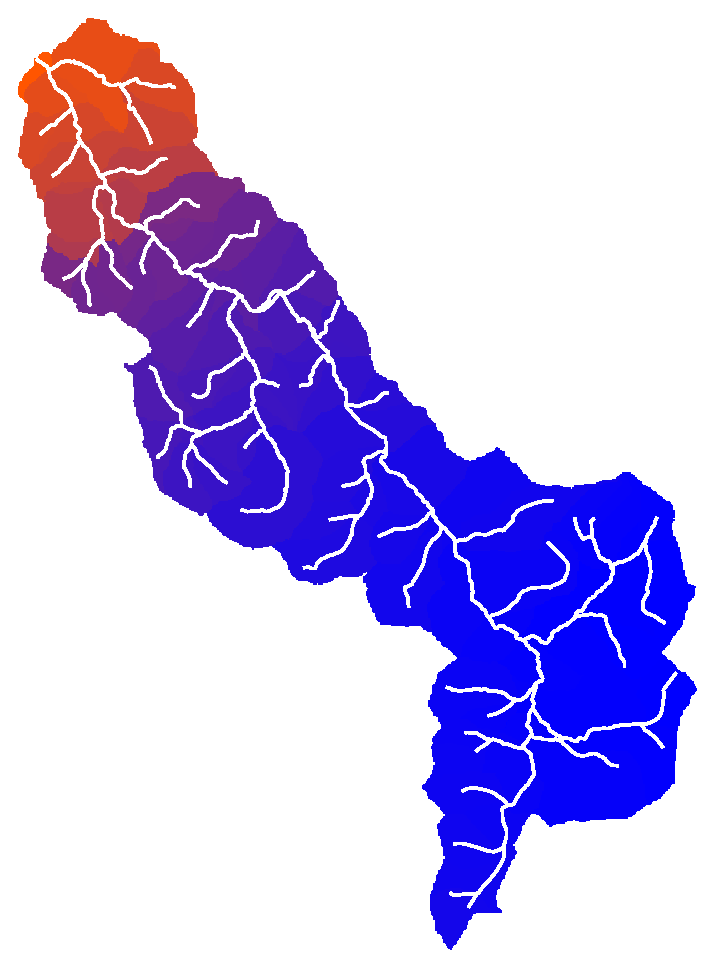
\includegraphics[width=0.3\textwidth, viewport=0 0 326 448, clip]{\figdir/demo/residInt_OFF.eps}
  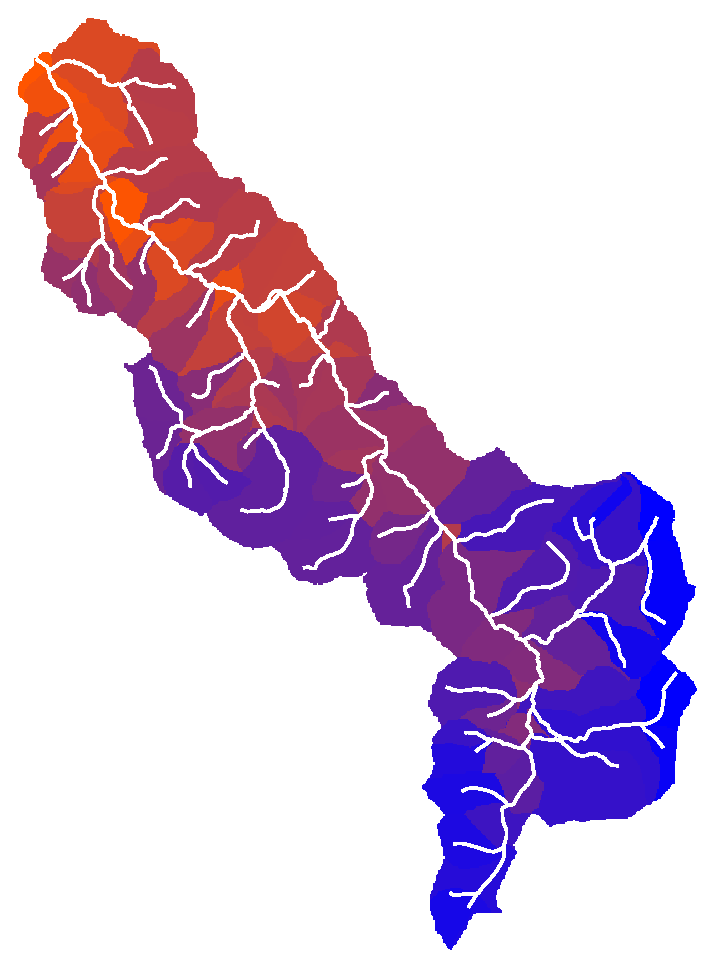
\includegraphics[width=0.3\textwidth, viewport=0 0 326 448, clip]{\figdir/demo/residInt_ON.eps}
  \caption[Example to illustrate the effect of residual interpolation.]{Effect of residual interpolation on the regionalization of air temperature in a mountainous watershed. In this example, the air temperature observed at climate stations is highly correlated to elevation. The stations (not shown) are located outside the watershed in the North (low elevation, warm) and South-East (high elevation, cold). Left: Elevation model (red: high, green: low) and river net (white). Center: \software{meteofill} output using the plain inverse-distance approach (blue: cold, red: warm). Right: \software{meteofill} output using residual interpolation with elevation as additional predictor. Obviously, higher temperatures are predicted in the valleys by taking the vertical temperature gradient into account. \label{fig:meteofill:resid}}
\end{figure*}

%%%%%%%%%%%%%%%%%%%%%%%%%%%%%%%%%%%%%%%%%%%%%%%%%%%%%%%%%%%%%%%%%%%%%%%%%%%%%%%%
%%%%%%%%%%%%%%%%%%%%%%%%%%%%%%%%%%%%%%%%%%%%%%%%%%%%%%%%%%%%%%%%%%%%%%%%%%%%%%%%
%%%%%%%%%%%%%%%%%%%%%%%%%%%%%%%%%%%%%%%%%%%%%%%%%%%%%%%%%%%%%%%%%%%%%%%%%%%%%%%%
\section{Arguments and invocation of \software{meteofill}} \label{sec:meteofill:args}

\software{meteofill} is an application written in C++. It expects all input to be supplied as command line arguments. All arguments must be supplied in a keyword-values style as in the following example call:

\begin{lstlisting}[style=shell]
meteofill ifile_locations="locations.txt"
  ifile_data="data_withGaps.txt"
  chars_colsep=" " chars_comment="#"
  nodata=-99. idw_power=2
  nsectors=4 norigins=3
  resid_nmin=3 resid_r2min=0.36
  resid_llim=-40. resid_ulim=40.
  ofile_data="data_filled.txt"
  ofile_locations="locations.txt"
  ndigits_max=1 logfile="log.txt"
  overwrite=true
\end{lstlisting}

The meaning of the various keywords is as follows:

\begin{columndef}
  \item[ifile\_locations] (\textit{string}) Input file listing the spatial coordinates for all locations. See \secref{sec:meteofill:input:locationsTable} for details.
  \item[ifile\_data] (\textit{string}) Input file with multi-location time series data. See \secref{sec:meteofill:input:timeSeries} for details.
  \item[chars\_colsep] (\textit{character(s)}) One or more character(s) used as a column-separator. Should be quoted, if a special character like TAB (ASCII code 9) is used. Any of the characters (if more than one) is treated as a column separator when reading input files. The columns of output files are separated by the first (or only) character in the set. Typically, a TAB character (enclosed by quotes) is used as in the above example.
  \item[chars\_comment] (\textit{character}) Initial character of comment lines in input files (typically the hash character). Should be quoted.
  \item[nodata] (\textit{numeric}) Value to indicate a missing value in the input time series. Typically, large negative values like -99 or -9999 are used for the common meteorological variables.
  \item[idw\_power] (\textit{numeric}) Value of parameter $p$ in \eqnref{eqn:meteofill:idw}. Typically a value of 1 or 2. The optimum value may be determined by cross-validation or variogram analysis.
  \item[nsectors] (\textit{integer}) Number of sectors to be used in the search of source locations (see \figref{fig:meteofill:nearest}). Using \texttt{nsectors=1} forces a nearest-neighbor interpolation. You probably want to use a value between 3 and 8 (or 1).
  \item[norigins] (\textit{integer}) The number of sector origins (sector rotations) to be tested. See \secref{sec:meteofill:idw} (\figref{fig:meteofill:rotation}). You probably want to use a value between 1 and 5. Larger values should give better results at the expense of an increase in computation time.
  \item[resid\_nmin] (\textit{integer}) Minimum number of locations with valid data (source locations) for possibly activation of residual interpolation. If the actual number of source locations is less than \verb!resid_nmin!, residual interpolation is \emph{not} used. Otherwise, the decision depends on the quality of the linear correlation (see \verb!resid_r2min!). Reasonable values for \verb!resid_nmin! are probably $\ge$ 3.
  \item[resid\_r2min] (\textit{numeric}) Minimum $R^2$ of the linear model used in residual interpolation (see \secref{sec:meteofill:resid}). For actual activation of residual interpolation, the computed $R^2$ for the particular time step must be $ge$ \verb!resid_r2min! and, \emph{in addition}, the sample size must be large enough (see \verb!resid_nmin!). Reasonable values for \verb!resid_r2min! are probably $\ge$ 0.36 (correlation coefficient of 0.6).
  \item[resid\_llim] (\textit{numeric}) Lower truncation limit in case of residual interpolation (see \secref{sec:meteofill:resid}). For variables that cannot take negative values (like precipitation or short-wave radiation), \verb!resid_llim! should be set to zero.
  \item[resid\_ulim] (\textit{numeric}) Upper truncation limit in case of residual interpolation (see \secref{sec:meteofill:resid}).
  \item[ofile\_data] (\textit{string}) Name/path of the output file containing the time series with all gaps filled according to the method described in \secref{sec:meteofill:method}.
  \item[ofile\_locations] (\textit{string}) Name/path of the output file containing a list of the locations from \verb!ifile_locations! for which data are actually present in \verb!ifile_data!.
  \item[logfile] (\textit{string}) Name/path of an output log file.
  \item[ndigits\_max] (\textit{integer}) Number of digits to be used in the output file \verb!ofile_data!.
  \item[overwrite] (\textit{logical}) A value of either true of false. If true, any existing output files will silently be replaced.
\end{columndef}

After successful execution, the return code of \software{meteofill} is zero. If the program terminates due to an error, a non-zero code is returned and traceback info is sent to standard output.

%%%%%%%%%%%%%%%%%%%%%%%%%%%%%%%%%%%%%%%%%%%%%%%%%%%%%%%%%%%%%%%%%%%%%%%%%%%%%%%%
%%%%%%%%%%%%%%%%%%%%%%%%%%%%%%%%%%%%%%%%%%%%%%%%%%%%%%%%%%%%%%%%%%%%%%%%%%%%%%%%
%%%%%%%%%%%%%%%%%%%%%%%%%%%%%%%%%%%%%%%%%%%%%%%%%%%%%%%%%%%%%%%%%%%%%%%%%%%%%%%%
\section{Input} \label{sec:meteofill:input}

\subsection{Locations table} \label{sec:meteofill:input:locationsTable}
The locations table is a text file with four columns (see \secref{sec:meteofill:args} for how to select a column separator). The expected column names are \texttt{id}, \texttt{x}, \texttt{y}, and \texttt{z}. The \texttt{id} column contains the names of locations (usually climate stations or rain gages), for which data are available. The IDs are read as strings. The corresponding spatial coordinates go in the \texttt{x} and \texttt{y} fields. For the coordinates one should use a \emph{geodetic} system (\ie{} units of meters, kilometers, miles, etc.). The \texttt{z} field should contain the values of the external predictor variable for residual interpolation. Elevation is the natural choice if nothing better is available. If residual interpolation should not be used anyway, the \texttt{z} column may be filled with dummy values.

An example of a locations table is given in \figref{fig:meteofill:input:locationsTable}.

\begin{figure}
\begin{lstlisting}[style=txt]
id	x	y	z
klotzsche	4623183	5667440	227
hosterwitz	4629789	5655359	114
strehlen	4623996	5652991	119
dipps_rein	4620226	5644000	365
zinnwald	4623539	5622933	877
\end{lstlisting}
  \caption{Example of a locations table. \label{fig:meteofill:input:locationsTable}}
\end{figure}

It is OK if the locations table contains more than the mandatory columns. \software{meteofill} simply ignores the unnecessary information. It is also OK if the locations table contains records for additional locations not present in the time series input file (\secref{sec:meteofill:input:timeSeries}). These records are silently ignored as well.

\subsection{Time series file} \label{sec:meteofill:input:timeSeries}
The time series input file is a text file with $n+1$ columns where $n$ is the number of locations (see \secref{sec:meteofill:args} for how to select a column separator). The table must have a header line with column names.
The first column of the file is expected to contain time information in ascending order (oldest record first). Any format can be used as \software{meteofill} internally treats the data as strings, not as times. For this first column, an arbitrary name can be chosen (but it must be present).
The remaining $n$ columns contain the numeric observation data at the $n$ locations. These columns may be in any order but their names need to match exactly with the location IDs provided in the locations table (\secref{sec:meteofill:input:locationsTable}). Any missing or invalid data values must be indicated by the \texttt{nodata} value (see \secref{sec:meteofill:args}). An example of multi-location time series file is given in \figref{fig:meteofill:input:timeSeries}.

\begin{figure}
\begin{lstlisting}[style=txt]
time	MT.CMP.	ARIES	MT.ORO
2000-01-01	0	-99	0
2000-01-02	4	-99	1
2000-01-03	12	3	1
2000-01-04	-99	-99	-99
2000-01-05	0	-99	0
\end{lstlisting}
  \caption{Example of multi-location time series file for use with \software{meteofill}. \label{fig:meteofill:input:timeSeries}}
\end{figure}

For the algorithm to be successful, it is important that the very first (oldest) record contains valid data for one location, at least.

%%%%%%%%%%%%%%%%%%%%%%%%%%%%%%%%%%%%%%%%%%%%%%%%%%%%%%%%%%%%%%%%%%%%%%%%%%%%%%%%
%%%%%%%%%%%%%%%%%%%%%%%%%%%%%%%%%%%%%%%%%%%%%%%%%%%%%%%%%%%%%%%%%%%%%%%%%%%%%%%%
%%%%%%%%%%%%%%%%%%%%%%%%%%%%%%%%%%%%%%%%%%%%%%%%%%%%%%%%%%%%%%%%%%%%%%%%%%%%%%%%
\section{Output} \label{sec:meteofill:output}
The current version of \software{meteofill} generates three output files whose names are specified at the command line (see \secref{sec:meteofill:args}). The contents of the files is described in \tabref{tab:meteofill:output}.

\begin{table*}
  \caption[Output files of \software{meteofill}.]{Output files of \software{meteofill}. The entries in the 'File' column refer to the command line arguments describe in \secref{sec:meteofill:args}. \label{tab:meteofill:output}}
  \begin{tabular}{p{0.2\textwidth} p{0.75\textwidth}} \hline\hline
    File & Contents \\ \hline
    \verb!ofile_data! & A multi-location time series table. Format and contents are identical to the input time series \secref{sec:meteofill:input:timeSeries} except that all \texttt{nodata} values are replaced by estimates according to \secref{sec:meteofill:method}. \\
    \verb!ofile_locations! & Similar to the input locations table described in \secref{sec:meteofill:input:locationsTable}. The table contains only the mandatory columns and list only those stations for which time series data are actually present. \\
    \verb!logfile! & Lists, for each time step, the number of locations with valid data (as absolute number in column \texttt{numdata} and as a percentage in column \texttt{availability}. The column \texttt{config\_changed} contains information on whether the set of locations with missing data has changed in comparison to the previous time step (requiring a new search for neighbored locations). The columns \texttt{residual\_interp} and \texttt{r2} contain information on the use of residual interpolation (true/false) and the corresponding $R^2$ of the linear model. \\ \hline\hline
  \end{tabular}
\end{table*}

%%%%%%%%%%%%%%%%%%%%%%%%%%%%%%%%%%%%%%%%%%%%%%%%%%%%%%%%%%%%%%%%%%%%%%%%%%%%%%%%
%%%%%%%%%%%%%%%%%%%%%%%%%%%%%%%%%%%%%%%%%%%%%%%%%%%%%%%%%%%%%%%%%%%%%%%%%%%%%%%%
%%%%%%%%%%%%%%%%%%%%%%%%%%%%%%%%%%%%%%%%%%%%%%%%%%%%%%%%%%%%%%%%%%%%%%%%%%%%%%%%
\section{Hints for practical usage} \label{sec:meteofill:hints}

\subsection{Missing-only data (options beyond persistence)} \label{sec:meteofill:hints:persistenceOptions}
As pointed out in \secref{sec:meteofill:filling}, \software{meteofill} assumes persistence if, in a particular time step, no data are available for any station (let's call this situation a \emph{global gap}). Although persistence is a simple and intuitive approach, it is likely to give satisfactory results only as long as the period of missing-only data is short enough. For long-lasting global gaps, persistence may not be a suitable assumption and it may be desireable to fill the gap with predefined values. Possible candidates are monthly average values or, in the case of rainfall data, a fixed value of zero.

Furtunately, there is a simple trick to let \software{meteofill} fill such global gaps with predefined values. All you need to do is to supplement the input data with a \emph{synthetic} station that 'recorded' the desired fill-in values (which may vary in time). The spatial coordinates of that synthetic station must be chosen so that it is \emph{very far} away from all the actual stations (\eg{} some million kilometers). Hereby it is ensured that the data from the synthetic station will practically be ignored (\ie{} weighted with almost zero), as long as any of the actual stations provides valid data.
